\section{Appendix}
\subsection{Upper Body Skeleton}
\noindent
The skeleton and the corresponding names for each joint for the upper body are illustrated in Figure \ref{fig:upper_body_skeleton} and Table \ref{table:upper_body_joint_names} respectively. There are 8 keypoints.
\begin{table}[ht]
\begin{minipage}[b]{0.60\linewidth}
\centering
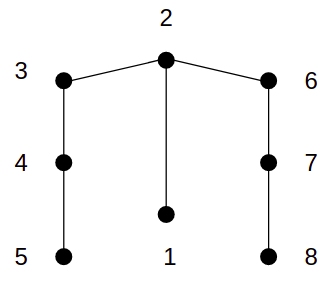
\includegraphics[width=250px]{assets/upper_body_skeleton.png}
\captionof{figure}{Upper Body Skeleton}
\label{fig:upper_body_skeleton}
\end{minipage}
\begin{minipage}[b]{0.35\linewidth}
\centering
\begin{tabular*}{\textwidth}{ c @{\extracolsep{\fill}} p{1.5in}}
Index & Joint Name \\ \hline
1 & Spine  \\ 
2 & Neck  \\ 
3 & Right Shoulder  \\ 
4 & Right Elbow  \\ 
5 & Right Wrist  \\ 
6 & Left Shoulder  \\
7 & Left Elbow  \\ 
8 & Left Wrist  \\ 
\end{tabular*}
\caption{Upper Body Joint Names}
\label{table:upper_body_joint_names}
\end{minipage}\hfill
\end{table}
\newpage

\subsection{Hand Skeleton}
\noindent
The skeleton and the corresponding names for each joint for the hand are illustrated in Figure \ref{fig:hand_skeleton} and Table \ref{table:hand_joint_names} respectively. There are 21 keypoints.
\begin{table}[ht]
\begin{minipage}[b]{0.60\linewidth}
\centering
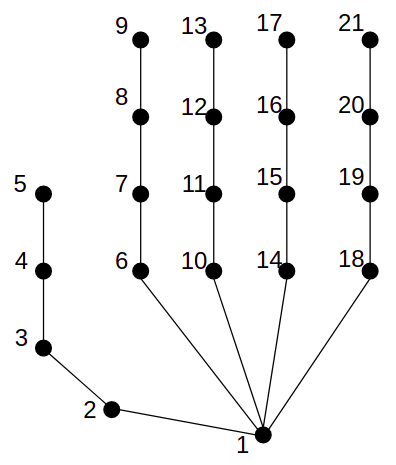
\includegraphics[width=250px]{assets/hand_skeleton.png}
\captionof{figure}{Hand Skeleton}
\label{fig:hand_skeleton}
\end{minipage}
\begin{minipage}[b]{0.35\linewidth}
\centering
\begin{tabular*}{\textwidth}{ c @{\extracolsep{\fill}} p{1.5in}}
Index & Joint Name \\ \hline
1 & Wrist  \\ 
2 & Thumb 1  \\ 
3 & Thumb 2  \\ 
4 & Thumb 3  \\ 
5 & Thumb 4  \\ 
6 & Index 1  \\
7 & Index 2  \\ 
8 & Index 3  \\ 
9 & Index 4  \\ 
10 & Middle 1   \\ 
11 & Middle 2  \\ 
12 & Middle 3  \\ 
13 & Middle 4  \\ 
14 & Ring 1  \\
15 & Ring 2  \\ 
16 & Ring 3  \\ 
17 & Ring 4  \\ 
18 & Pinky 1  \\ 
19 & Pinky 2  \\ 
20 & Pinky 3  \\ 
21 & Pinky 4  \\ 
\end{tabular*}
\caption{Hand Joint Names}
\label{table:hand_joint_names}
\end{minipage}\hfill
\end{table}